As described earlier, subtopic clustering has always been a challenging task in information retrieval field. The subtopic retrieval method developed by Bernardini et al. is limited by several factors: 
\begin{itemize}
    \item It is highly dependent on keyphrases generated from the search results
    \item In high precision scenario where our candidate set size is small, it will be difficult to generate useful keyphrases
    \item Their method is evaluated with a non-standard evaluation metric
\end{itemize}
Hence we feel, the problem of subtopic clustering requires a generic solution which can be verified by standard clustering metrics. Transformer based embedding model brings not only simplicity, efficiency and generality of an embedding model but also the ability to capture complex semantic information. Both of these features are necessary key-ingredients to solve challenging IR problems such as subtopic clustering. Our main focus in this section is to use these embeddings as key ingredients and find simple modifications that can capture subtopic similarity between passages related to a topic and thus can cluster them based on those subtopics.

\subsection{Basic steps to subtopic clustering} We model subtopic clustering task as a pairwise distance learning problem. Any subtopic clustering problem can be solved by two basic steps:
\begin{itemize}
    \item Step 1: Estimate a pairwise supervised distance between all passage pairs.
    \item Step 2: Use Hierarchical Agglomerative clustering with the pre-computed pairwise distance to generate clusters of passages.
\end{itemize}

We focus on Step 1 to develop a suitable pairwise similarity metric between passages.

\subsection{Transformer embeddings} In their Sentence-BERT work, authors generate fixed length embeddings for a given word sequence. Dor et al. \cite{dor2018learning} propose a triplet fine-tuning technique which trains the embeddings to be better suited in predicting similarity of sentence pairs based on their likeliness of sharing same section in an Wikipedia article. Each training example consists of one anchor sentence, one similar sentence which is from same section than the anchor and one dissimilar sentence which is from different section than anchor. Using each of these approaches, we obtain fixed length embeddings for passages using tokenized passages as input token sequence. A straight-forward approach for the subtopic clustering would use cosine similarity between these fixed-length vectors as to quantify the pairwise similarity between passages. The similarity scores are used in  a clustering algorithm to obtain subtopic clusters. Note that, transformer models have a maximum input length. So for longer passages tokens beyond the maximum length are truncated.

Although the triples data and target task proposed by Dor et al. may help detect a sentence pair from from the same subtopic (i.e., same section of Wikipedia), we hypothesize that without certain modifications specific to subtopic clustering, we obtain sub-optimal results. There are several reasons behind our hypothesis: 
\begin{itemize}
    \item Natural sentences are shorter than paragraph-sized \ld{I added paragraph-sized, because some IR folks think that passages are sentences} passages and henceforth, it is hard to find sentences with much topical drifts. So there is hardly any ambiguity in deciding the central topic discussed \ld{I don't understand what you mean by article:} in an article. So the target task for sentence-pair similarity is to decide whether the specific topics discussed in each sentences of the pair is associated with the same section or they are distinct enough to be associated with different sections \ld{the section and article terminology would either need to be introduced earlier or we would need to explain this in terms of general terms like subtopics} of an article. For passage-pair however it is much more difficult because constituent sentences in a passage may be of different fine-grained topic.
    \item Wikipedia articles are organized in hierarchical sections; passages deeper in the hierarchy tend to discuss more specific topics than passages on a higher level. Hence two passages which share the same top-level section but belong to different deeper level sections may provide ambiguous supervision signals if used as training examples. This hierarchical ambiguity in training data generation is not considered in the method of Dor et al. which may result to undertrained model if adapted for subtopic clustering of passages.
    \item As any subtopic clustering is highly query dependent, we hypothesize that an accurate subtopic similarity metric must take the user's query (or other expressions of the information need) into consideration.
\end{itemize}

We propose the following simple modifications to the previous approaches when applied to subtopic clustering:
\begin{itemize}
    \item Due to the reason discussed above, while generating negative \ld{I replace dissimilar with negative, your choice} training-examples for passage triples, we only consider passages which are from a different top-level branches in the hierarchy than the anchor passage. This will provide clear, unambiguous and distinguishable supervision signal to the model under fine-tuning and help it to quickly learn the desired similarity function. Figure \ref{fig:conv} depicts the training data generation.
    \item We train a query-dependent shallow network to provide pairwise passage similarity scores which are used by subsequent clustering algorithm to generate subtopic clusters of passages. Next we discuss this approach in more detail.
\end{itemize}{}
\begin{figure}[h]
  \centering
  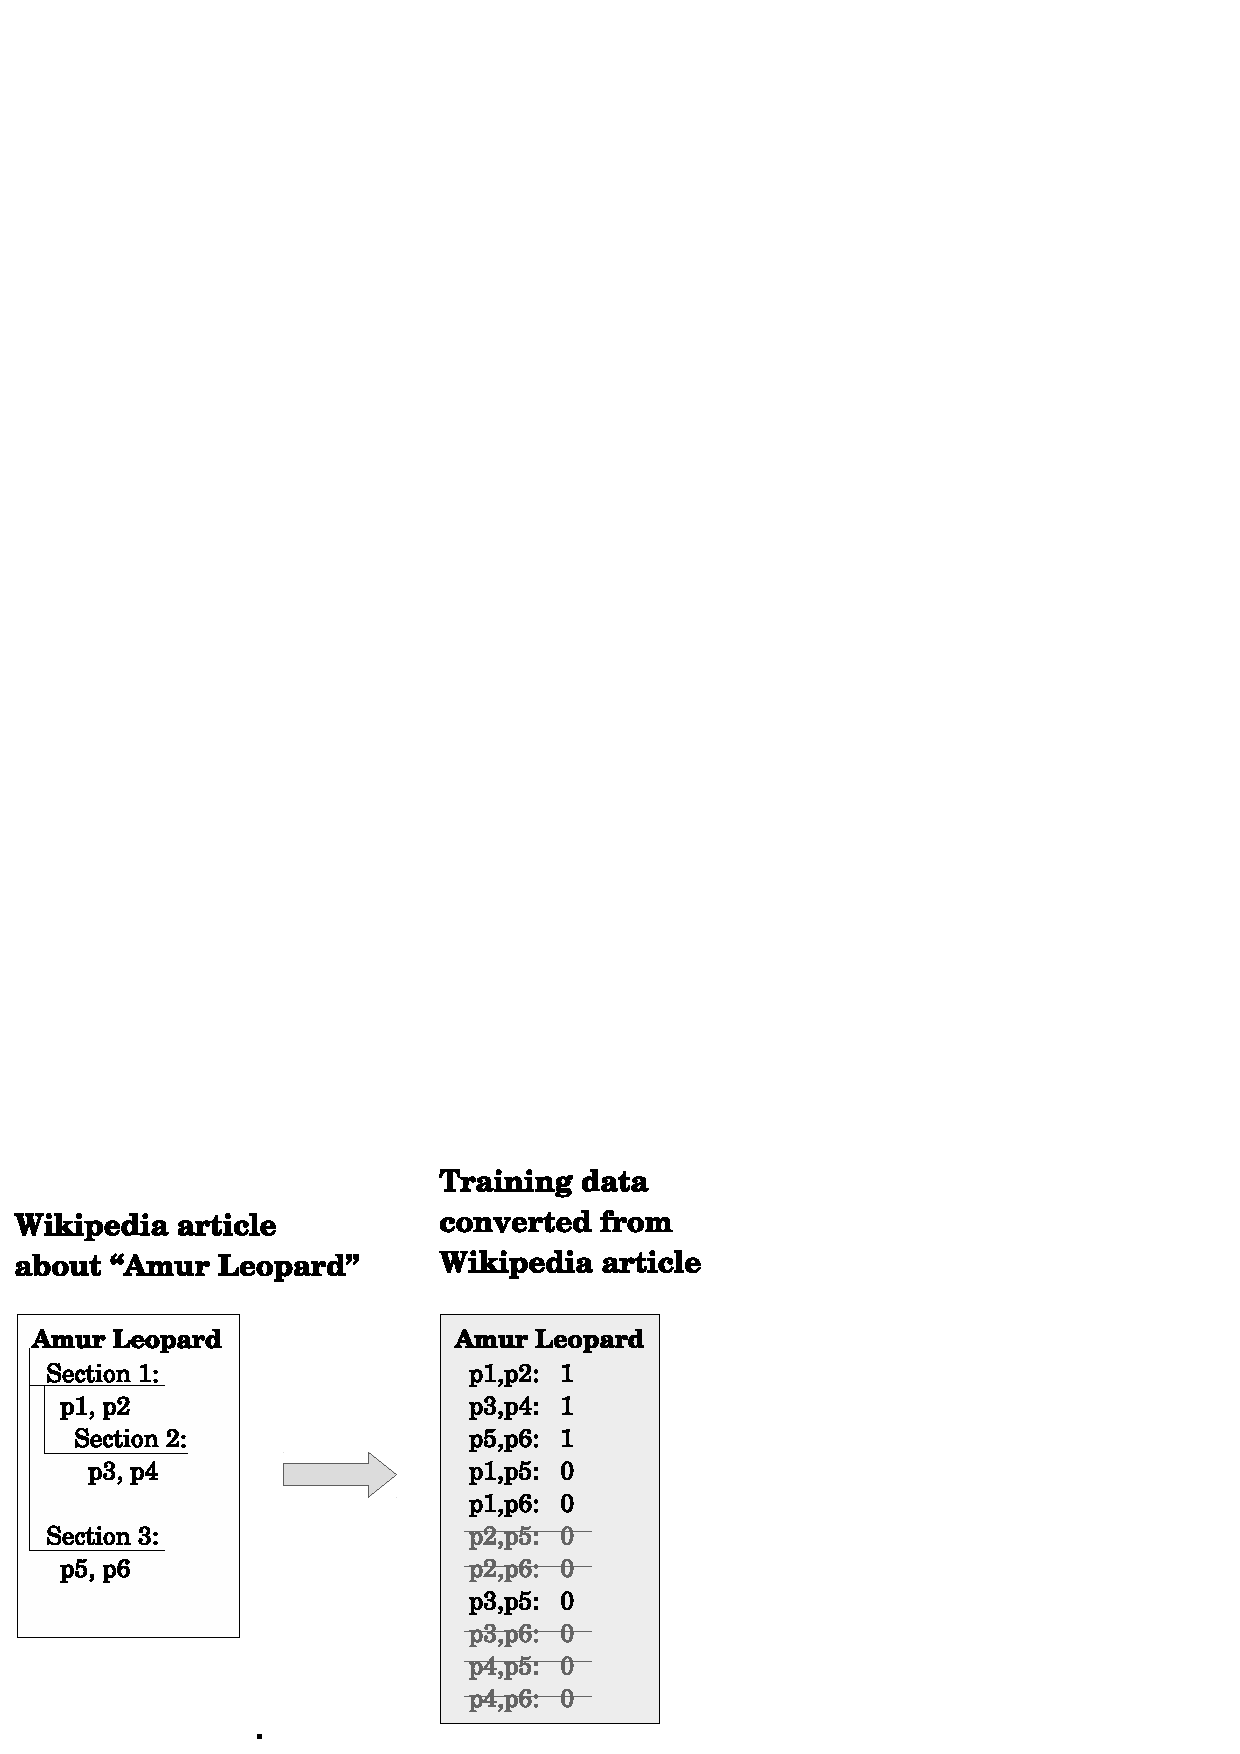
\includegraphics[width=\linewidth]{graphics/car_y1_conv.png}
  \caption{Training data generation from Article \textit{Amur Leopard} and balancing the dataset (depicted in grey strikethrough)}
  \label{fig:conv}
\end{figure}

\subsection{CATS: Context Aware Triamese Similarity network}\label{sec:cats} 
The similarity between a pair of texts is often subject to the context. In context of \textit{endangered species}, a pair of passages about \textit{Amur leopard} and \textit{Vaquita porpoise} should be considered similar. However this is not the case if the context changes to \textit{bycatch}. In subtopic clustering problems, context plays an important role in deciding whether passages about same broad topic should share the same subtopic cluster or not. Keeping this in mind, we propose CATS, Context Aware Triamese Similarity network, a triamese shallow network which learns a similarity function between a pair of passage embeddings in the context of a third embedding vector that represents the query or context information. For our application, we use the topic title as our contextual information need.

As depicted in Figure \ref{fig:triam}, the general CATS architecture consists of three identical fully connected triamese neural layers ($DL1$), meaning they share the same set of weights. Each of them accepts fixed-length embedding vectors representing the query context and pair of passages respectively ($u,v,w$) \ld{which variable is the query? the sentence? would it help to call them $\vec{q}, \vec{s_1} and \vec{s_2}$ ?}. Due to their triamese nature, they project all three embedding vectors to the same embedding subspace. The projected vectors ($u',v',w'$) and their difference vectors ($(v'-w'),(v'-u'),(w'-u')$) are concatenated. The concatenated output vector is transformed through another fully connected neural layer ($DL2$) which emits a similarity score.
\begin{figure}[h]
  \centering
  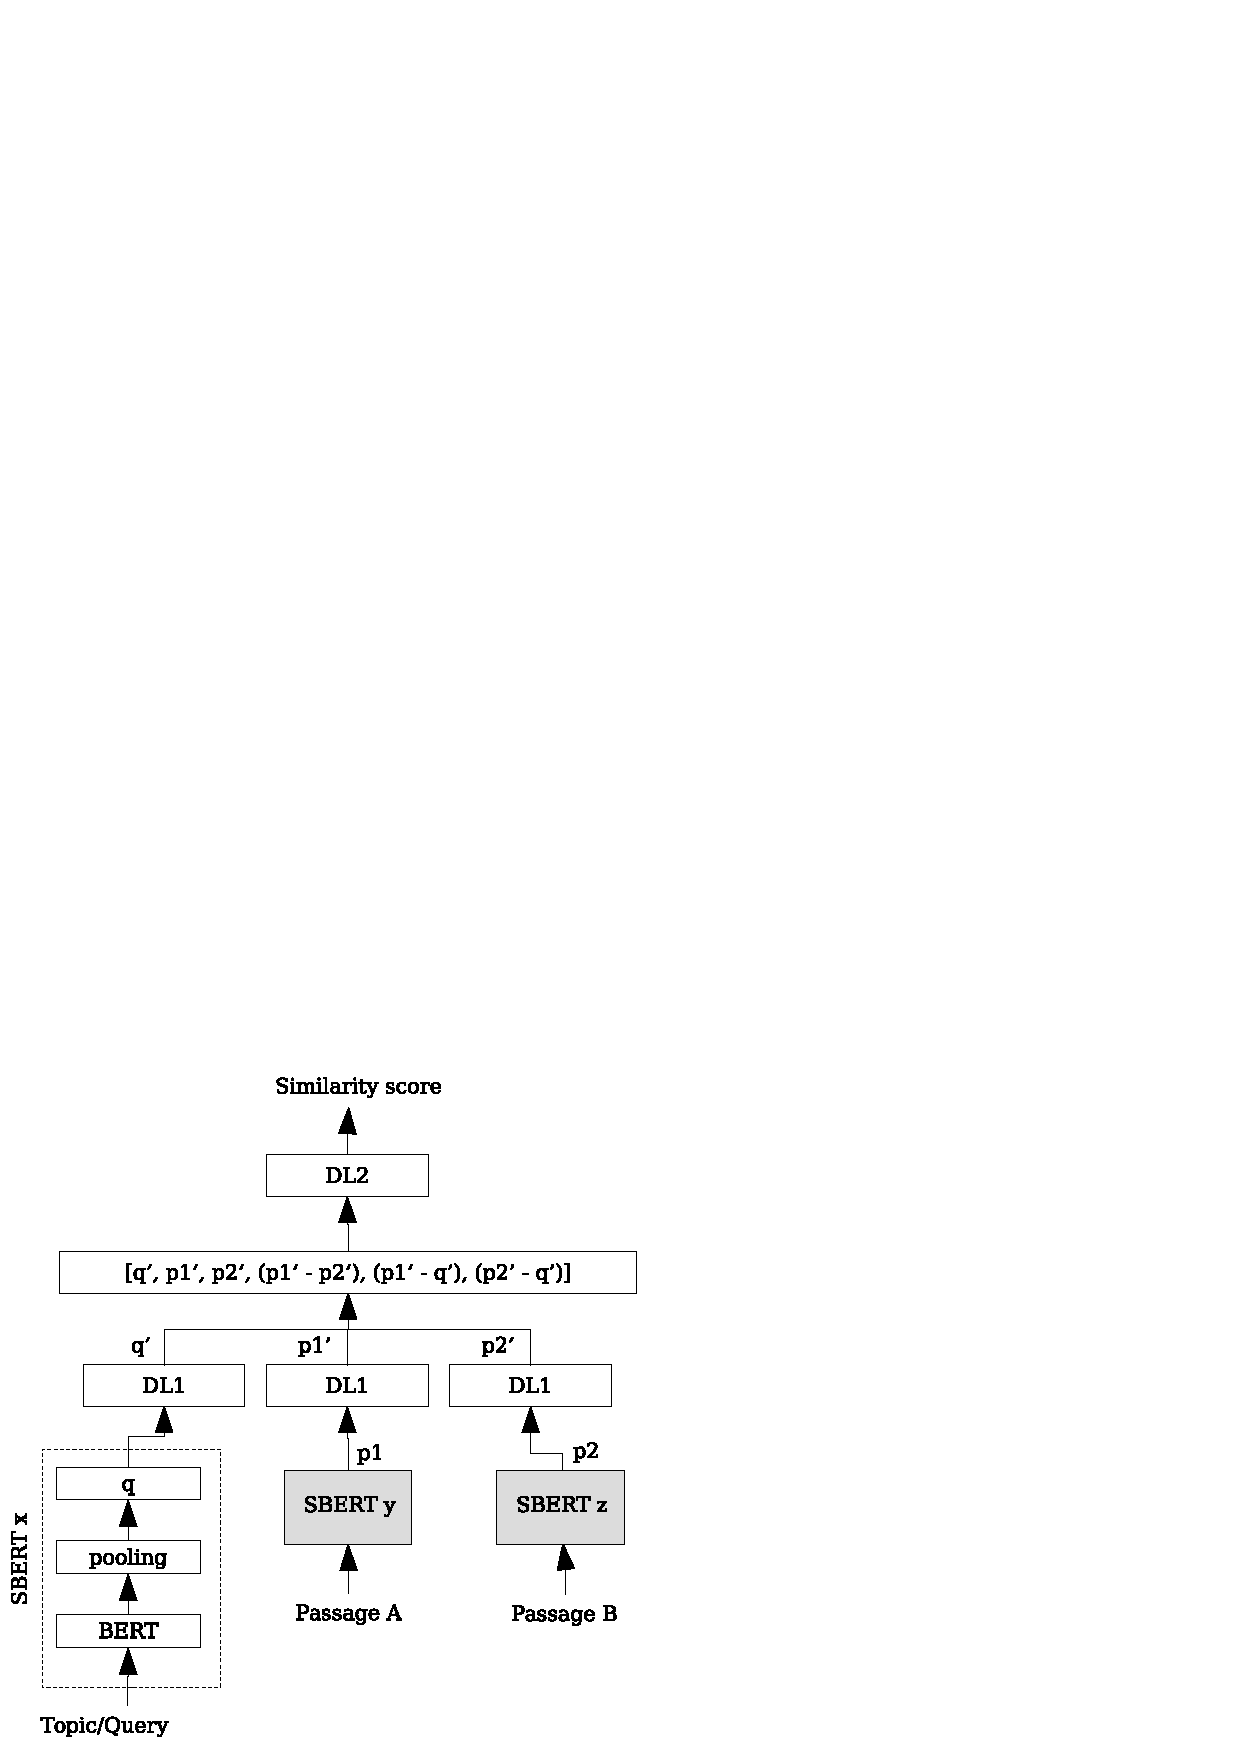
\includegraphics[width=\linewidth]{graphics/triamese.png}
  \caption{Triamese network used to estimate query dependent pairwise passage similarity score used for subtopic clustering}
  \label{fig:triam}
\end{figure}

\subsection{Finetuning transformers for sequence pair tasks} Fine-tuning is a crucial step in training Transformer models because this allows the model to be specifically suited for a particular downstream task. In the original BERT work, the BERT model is fine-tuned for a binary classification task with STSB benchmark dataset \ld{citation needed}. In that work BERT model is fine-tuned for next sentence prediction task where given a sentence-pair, the model has to predict whether the second sentence should follow the first sentence. We fine-tune the  \ld{earlier you capitalized Transformer} transformer with a modified task: given a passage-pair, predict whether they should belong to the same subtopic. This modified task setting allows us to use output of the model as the similarity score between the input passages. However, our focus for this work is to explore the benefits of fixed-length passage embeddings and hence use this technique only as a strong baseline against our embedding based methods.